\documentclass[a4paper]{article}

%% Language and font encodings
\usepackage[english]{babel}
\usepackage[utf8x]{inputenc}
\usepackage[T1]{fontenc}

%% Sets page size and margins
\usepackage[a4paper,top=3cm,bottom=2cm,left=3cm,right=3cm,marginparwidth=1.75cm]{geometry}

%% Useful packages
\usepackage{amsmath}
\usepackage{graphicx}
\usepackage[colorinlistoftodos]{todonotes}
\usepackage[colorlinks=true, allcolors=blue]{hyperref}
\usepackage{subfigure}
\usepackage{caption}
\usepackage{amsfonts}
\usepackage{amsthm}
\usepackage{upquote}
\usepackage{listings}
\usepackage{enumitem}
\usepackage{dirtytalk}
\usepackage{hyperref}
\usepackage{float}

\def\therefore{\boldsymbol{\text{ }
\leavevmode
\lower0.4ex\hbox{$\cdot$}
\kern-.5em\raise0.7ex\hbox{$\cdot$}
\kern-0.55em\lower0.4ex\hbox{$\cdot$}
\thinspace\text{ }}}

\title{A Journey to the Interactive 3D Fractal World}
\author{CSED Yang Junha 20160785, Ryu Sangwoo 20160845, Sung Haebin 20160463}

\begin{document}
\maketitle
\section{Summary}
This project is about rendering 3D fractals in an interactive, real-time-processing way.
We persue both aesthetic achievement, and optimized, well-programmed rendering pipeline as well.
\section{Motivation}
Fractals are so beautiful.
We can see tons of fractal videos on Youtube, and many people get inspiration from such elegant mathematical geometry.
But we realized that it could be even more better with real-time interaction.
\section{What to do}
\say{A Journey to the Interactive 3D Fractal World}, briefly speaking.
\subsection{High Resolution Fractals}
We will generate high resolution fractals without any pre-calculated textures.
Which means, it involves direct pixel-level calculation.
The mathematical fractal model we're going to use is not determined, but we're considering to start from a famous model, such as the Mandelbrot Set.
We can generate creative and unique new fractals from such well known fractal models, by distorting and adjusting some parameters.
Because fractals are so sensitve and fine-tuned, there lies a kind of butterfly effect around fractal world.
(Thus it requires delicate and exquisite calculations)
\subsection{3D Geometry}
Again, we will present a 3D fractal world.
The basic process of 3D viewing and transformation will of course be adopted, but there would be something more than that.
Some of the ideas are reordering viewing parameters, mixing or partially omitting some part of the pipeline, or many weird things.
Usage of hierarchical models could be also helpful, like what we saw in the midterm exam, but we would need more complex models than that.
\subsection{Animation}
Changing the parameters of fractal or camera would yield beautiful animation.
\subsection{Realtime Rendering and Interaction}
We particularly want to emphasize the spatial impression of fractal world (that's why this project is about 3D).
So wandering by yourself in the fractal world is essential to perceive the full structure of complex fractal space.
Therefore we aim to provide people the realtime-rendering experience rather than just a video after long-time processing,
meaning you can actually control the camera and do some action on the program.
\section{How to achieve}
\subsection{Development Enviornment}
In this project we need direct controlling of the shaders, especially fragment shaders.
Or even there could be some arbitrary change of pipeline in overall, because extreme features of fractal geometry could require some modification of typical graphics procedures.
And also one of our goal is about optimization of this particular task, so we consider low-level programming.

And fractals are not highly related to photo realism, so many pre-developed presets and modules provided by
graphics engines such as Unity won't be particularly helpful.
Thus we'll develop this project with pure OpenGL(with glut, glm, ...)
\subsection{Shaders}
The key idea of rendering fractals is using fragment shaders wisely.
'Escape-time fractals', such as Mandelbrot set is rendered based on the speed of diversion for every complex coordinates.
So those kinds of fractals will require the renderer to perform per-pixel calculation, which is the reason fragment shaders are for.

And vertex shaders are also important.
To construct 3D space of fractals, we should choose either voxel rendering or 3D polygons with 2D fractal textures.
Voxel is very intutive and expressive, but needs an enormous amount of calculation.
Thus we consider 3D polygons, but those polygons should be also complex and fractalistic enough.
We also expect an animation of fractal space, so vertex shaders also must be used well.
\subsection{Advanced Rendering Techniques}
Advanced techniques like shading, texture, arbitrary clipping, aliasing would make the final quality better or even produce some novel graphic.
Our lecture hasn't covered those topics yet, so we will think about this later.
\section{Notable References}
\subsection{Textbooks}
There are 3 reference textbooks we'll study.
\textit{Interactive Computer Graphics}\cite{c1}, our course textbook, introduces some background of fractal geometry and examples like Mandelbrot Set.
\textit{OpenGL SuperBible}\cite{c2} introduces rendering methods of Julia fractals using shader.
\textit{Rendering Methods for 3D Fractals}\cite{c3} introduces volume rendering methods for fractal rendering and methods for 3D Fractal high resolution image. We can choose techniques for 3D fractal calculation and rendering.

\subsection{Fragmentarium}
\textbf{Fragmentarium} is an open source, pixel-based graphics rendering tool, which is part of what we want to do.
The program's input script is based on GLSL, with some added functionalities and preprocessors.
Fragmentarium is good for generating fractal art, such as \url{https://www.flickr.com/groups/fragmentarium/}.
It is open source and based on GLSL shaders, so we think we could get something out of it.
You could get more details from \url{http://syntopia.github.io/Fragmentarium/index.html}.

\section{Gallery}
\begin{figure}[H]
\centering
\subfigure[scene from a Youtube video(\url{https://youtu.be/S530Vwa33G0})]
{
    \label{fig:subfig1}
    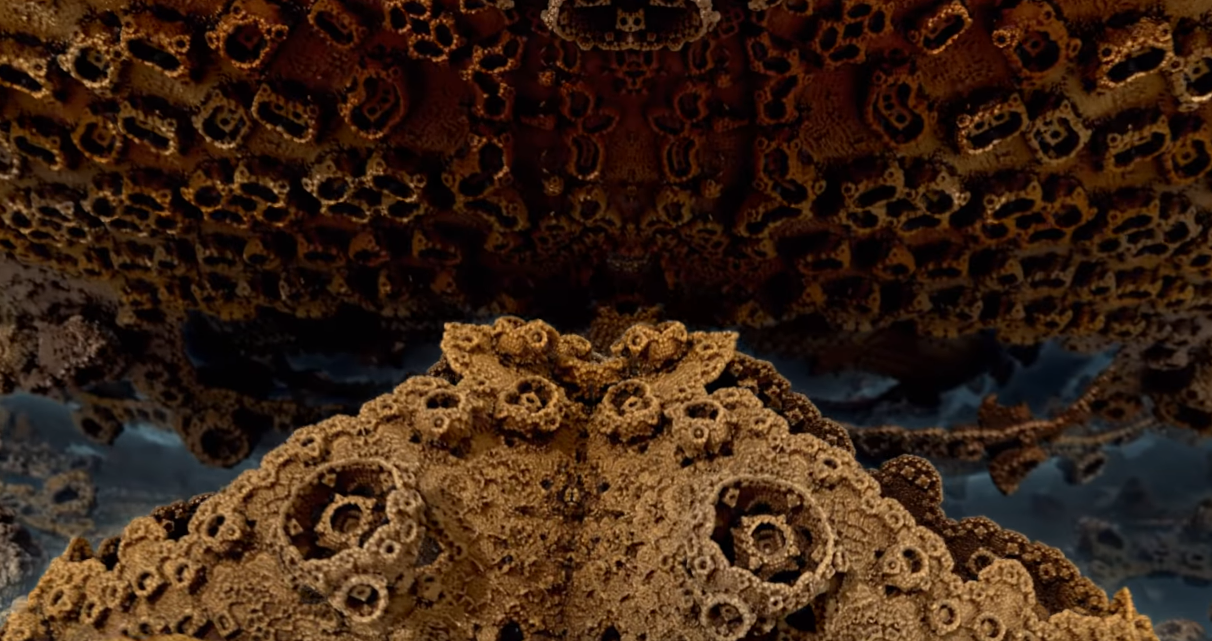
\includegraphics[scale=0.3]{cap1.PNG}
}
\end{figure}

\begin{figure}[H]
\centering
\subfigure[a Mandelbrot Set(\url{https://en.wikipedia.org/wiki/Mandelbrot_set})]
{
    \label{fig:subfig2}
    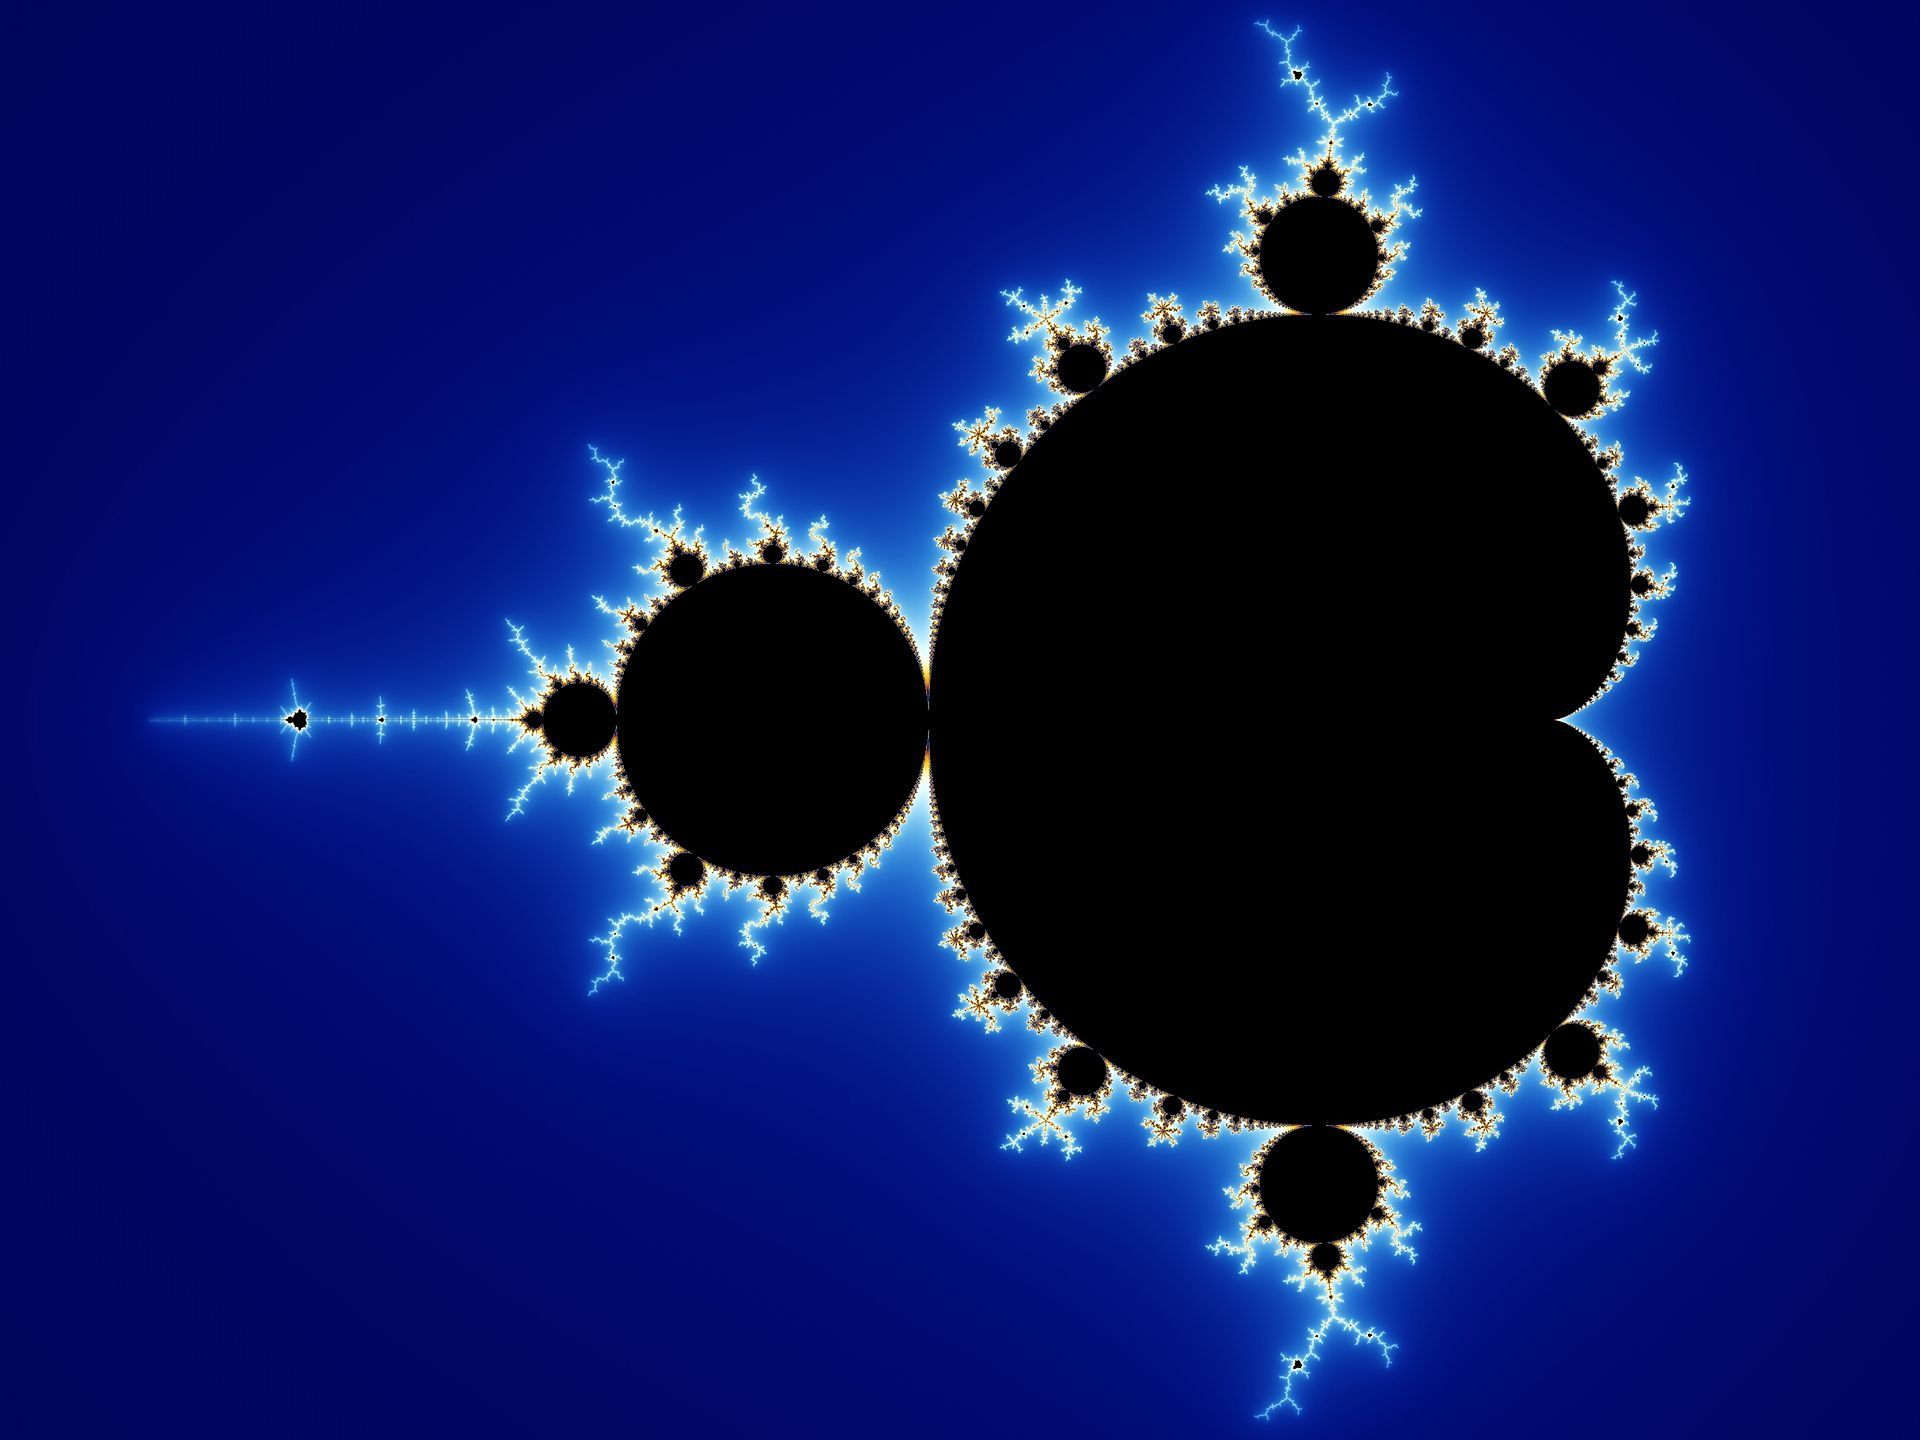
\includegraphics[scale=0.3]{mandel.jpg}
}
\end{figure}
\section{Discussion}
There are some issues in this project.
\begin{description}[style=nextline]
\item[Is rendering such high resolution 3D fractals possible in realtime?]
We agree that it's difficult generally, so some loss of quality could be inevitable.
But we believe most of the overhead can be optimized using very specialized techniques with a well-developed program.
\item[What level of achievement do we expect?]
Studying, researching and implementing all those features mentioned will be our goal.
The quality of product that we desire is slightly less than common fractal videos in Youtube, because we're doing in realtime. (search \say{3D fractal})
\item[What are our roles?]
Not clearly separated, but we have some background knowledge. Junha has exeperienced fractals before and familiar with machine learning. (Not sure if it is useful)
Sangwoo knows about dealing with videos(PBS). Haebin is good at low-level and system programming.
\end{description}

\begin{thebibliography}{1}
\bibitem{c1}E. Angel and D. Shreiner, Interactive Computer Graphics: A Top-Down Approach with Shader-Based OpenGL, 6th ed., Addison-Wesley, 2011, p.487 Section 9.8 Recursive Methods and fractals
\bibitem{c2}Graham Sellers; Richard S. Wright, Jr.; Nicholas Hanemel, OpenGL SuperBible, 7th ed., Addison-Wesley, p.683 Rendering Julia Fractals
\bibitem{c3}Rickard Englund, Rendering Methods for 3D Fractals
\textit{Science and Engineering Ethincs}, 2009, pp. 311-341.
\end{thebibliography}

\end{document}
